% Last update/Última versão: 11/Sep/2016
%%%%%%%%%%%%%%%%%%%%%%%%%%%%%%%%%%%%%%%%%%%%%%%%%%%%%%%%%%%%%%%%%%%%%%
%=====================================================================
% 							Pacotes Fundamentais
%=====================================================================
\documentclass[
% -- op\c{c}\~{o}es da classe memoir --
12pt,				% tamanho da fonte
openright,			% cap\'{\i}tulos come\c{c}am em p\'{a}g \'{\i}mpar (insere p\'{a}gina vazia caso preciso)
oneside,			% para impress\~{a}o em verso e anverso. Oposto a oneside
a4paper,		% tamanho do papel.
% -- op\c{c}\~{o}es da classe abntex2 --
%chapter=TITLE,		% t\'{\i}tulos de cap\'{\i}tulos convertidos em letras mai\'{u}sculas
%section=TITLE,		% t\'{\i}tulos de se\c{c}\~{o}es convertidos em letras mai\'{u}sculas
%subsection=TITLE,	% t\'{\i}tulos de subse\c{c}\~{o}es convertidos em letras mai\'{u}sculas
%subsubsection=TITLE,% t\'{\i}tulos de subsubse\c{c}\~{o}es convertidos em letras mai\'{u}sculas
% -- op\c{c}\~{o}es do pacote babel --
english,			% idioma adicional para hifeniza\c{c}\~{a}o
%french,			% idioma adicional para hifeniza\c{c}\~{a}o
%spanish,			% idioma adicional para hifeniza\c{c}\~{a}o
brazil,				% o \'{u}ltimo idioma \'{e} o principal do documento
%sumario=tradicional,
]{article}
\usepackage[a4paper, right = 2cm, left = 2.5cm, top = 3cm, bottom = 2cm]{geometry}
\usepackage[utf8]{inputenc}
\usepackage[english,portuguese]{babel}
%\usepackage[myheadings]{fullpage}
\usepackage[T1]{fontenc}
\usepackage{graphicx, setspace}
\usepackage{sectsty}
\usepackage{url}
%\usepackage{mathptmx} %% Para times
\usepackage{comment}
\usepackage{multirow}
\usepackage{graphicx}
\usepackage[table,xcdraw]{xcolor}
\usepackage{enumitem}
\usepackage{blindtext}
\usepackage{float}
\usepackage{tikz}
\usetikzlibrary{calc,trees,positioning,arrows,chains,shapes.geometric,%
	decorations.pathreplacing,decorations.pathmorphing,shapes,%
	matrix,shapes.symbols,through}
\usepackage[bottom]{footmisc}
\usepackage{pdfpages}
\usepackage{caption} % \caption*
\usepackage{csquotes}
\usepackage{footnote} % Permite footnote em tabelas
\renewcommand{\rmdefault}{phv} % Arial
\renewcommand{\sfdefault}{phv} % Arial


%=====================================================================
% 							Pacotes Bibliográficos
%=====================================================================

\usepackage[backend=biber,
	style = abnt,%
	noslsn, %
	extrayear, %
	uniquename=init,% 
	giveninits, %
	justify, %
	sccite,% 
	scbib, %
	repeattitles, %
	doi=false,isbn=false,url=false, 
	maxcitenames=3]{biblatex}
\addbibresource{../../Escrita_Dissertacao/Da_Silveira_Dissertacao_Atual/Bibliografia_Dissertacao/Bibliografia_Dissertacao.bib}
\addbibresource{../../Escrita_Dissertacao/Da_Silveira_Dissertacao_Atual/Fatos_Estilizados/Biblio.bib}

\renewenvironment{quote}
{\small\list{}{\fontsize{10pt}{12pt}\singlespacing\rightmargin=0cm \leftmargin=4cm}%
	\item\relax}
{\endlist}

%=====================================================================
% 							Comandos específicos da FAPESP
%=====================================================================
\newcommand{\HRule}[1]{\rule{\linewidth}{#1}}
\onehalfspacing
\setcounter{tocdepth}{3}
\setcounter{secnumdepth}{3}

\newcommand{\titulo}[1]{\def\meuTitulo{#1}}
\newcommand{\tituloIngles}[1]{\def\meuTituloIngles{#1}}
\newcommand{\numFAPESP}[1]{\def\numFAP{#1}}
\newcommand{\tipoRelatorio}[1]{\def\tipoRelat{#1 }} %o espaço depois do #1 é importante
\newcommand{\autor}[1]{\def\nomeAutor{#1}}
\newcommand{\cidade}[1]{\def\nomeCidade{#1}}
\newcommand{\universidade}[1]{\def\nomeUniversidade{#1}}
\newcommand{\faculdade}[1]{\def\nomeFaculdade{#1}}
\newcommand{\periodoVigencia}[1]{\def\periodVig{#1}}
\newcommand{\periodoRelatorio}[1]{\def\periodRelat{#1}}
\author{}
\date{}

\newcommand{\Figure}[1]{Figura~\ref{fig:#1}}
\newcommand{\Table}[1] {Tabela~\ref{#1}}
\newcommand{\Equation}[1] {Equa\c{c}\~ao~\ref{#1}}
\newcommand{\addFigure}[3] { %Parametros scale, fig_name, caption 
    \begin{figure}[!hbt]
      \centering
      \includegraphics[scale=#1]{figures/#2}
      \caption{#3}\label{fig:#2}
    \end{figure}
}

\newcommand{\geraTitulo}{
\clearpage
\begin{titlepage}
  \begin{center}
      \vspace*{-3cm}
      { \setstretch{.5} 
        \textsc{\nomeUniversidade} \\
        \HRule{.2pt}\\
        \textsc{\nomeFaculdade}
      }

      \vspace{5.5cm}

      \Large \textbf{\textsc{\meuTitulo}}
	  \HRule{1.5pt} \\ [0.5cm]
      \linespread{1}
      \large Relatório Científico \tipoRelat do Projeto de Auxílio à Pesquisa Regular, fomentado pela Fundação de Amparo à Pesquisa do Estado de São Paulo. \\ 
  	   \HRule{1.5pt} \\ [0.5cm]
       Projeto FAPESP \texttt{\#\numFAP}
       \\ [0.1cm]
       Pesquisador Responsável: \nomeAutor
       
       \vfill
       
       {\normalsize  \nomeCidade, \today}
\end{center}
\end{titlepage}
}

\usepackage{titlesec}
\titleformat{\chapter}{\normalfont\LARGE\bfseries}{\thechapter}{1em}{}
\titlespacing*{\chapter}{0pt}{3.5ex plus 1ex minus .2ex}{2.3ex plus .2ex}

%----------------------------------------------------------------------
% HEADER & FOOTER
%----------------------------------------------------------------------
\pagestyle{fancy}
\fancyhf{} % Limpa todos os campos de header and footer fields
%\setlength\headheight{15pt}
\renewcommand{\headrulewidth}{0pt}
%\fancyhead[R]{Anglia Ruskin University} 
\fancyfoot[R]{\thepage}%of \pageref{LastPage}}

\addto\captionsportuguese{\renewcommand{\contentsname}{Sumário}}
\addto\captionsportuguese{\renewcommand{\bibname}{Referências bibliográficas}}

%------
% Resumo e Abstract
%------
\newcommand{\Resumo}[1]{
   \begin{otherlanguage}{portuguese}
       \addcontentsline{toc}{chapter}{Resumo}
       \begin{abstract} \thispagestyle{plain} \setcounter{page}{2}
          #1
        \end{abstract}
   \end{otherlanguage} 
} %end \Resumo

\newcommand{\Abstract}[1]{
   \begin{otherlanguage}{english}
      \addcontentsline{toc}{chapter}{Abstract}
      \begin{abstract} \thispagestyle{plain} \setcounter{page}{3}
       #1
      \end{abstract}    
    \end{otherlanguage} 
} %end \abstract

%------
% Folha de rosto
%------
\newcommand{\folhaDeRosto}{
   \chapter*{Informações Gerais do Projeto}
   \addcontentsline{toc}{chapter}{Informações Gerais do Projeto}
   \begin{itemize}
      \item Título do projeto: 
            \begin{itemize}\item[] \textbf{\meuTitulo} \end{itemize}
      \item Nome do pesquisador responsável: 
            \begin{itemize}\item[]\textbf{\nomeAutor}\end{itemize}
      \item Instituição sede do projeto: 
            \begin{itemize}
               \item[]\textbf{\nomeFaculdade \ da \nomeUniversidade} 
            \end{itemize}
      \item Equipe de pesquisa:
            \begin{itemize}
               \item[]\textbf{\nomeAutor} 
            \end{itemize}
       \item Número do projeto de pesquisa:
            \begin{itemize}
               \item[]\textbf{\numFAP} 
            \end{itemize}
       \item Período de vigência:
            \begin{itemize}
               \item[]\textbf{\periodRelat} 
            \end{itemize}
       \item Período coberto por este relatório científico:
            \begin{itemize}
               \item[]\textbf{\periodVig} 
            \end{itemize}
   \end{itemize}
   \clearpage
}
%=====================================================================
% 							Outros Pacotes
%=====================================================================
\usepackage[colorinlistoftodos]{todonotes}
\usepackage{subfigure}
\usepackage{setspace}
\usepackage{lipsum}  
\usepackage{amsmath} % Para cases
%=====================================================================
% 							Página de título e folha de rosto
%=====================================================================
%-----
% Página de título
% Observação: As definições que aparecem a seguir comporão a
%             página de título e a folha de rosto.
%-----
%% Define o nome da universidade onde o projeto foi desenvolvido.
\universidade{Universidade Estadual de Campinas}
%
%% Define o nome da faculdade onde o projeto foi desenvolvido.
\faculdade{Instituto de Economia}
%
%% Define o título do projeto.
\titulo{Título}
%
%
%% Define o autor do relatório.
\autor{}
\cidade{Campinas}


\begin{document}
%=====================================================================
% 							Numeração pré-textual
%=====================================================================
\pagenumbering{roman}
%=====================================================================
% 							Folha de título
%=====================================================================
%\geraTitulo
%=====================================================================
% 							Folha de rosto
%=====================================================================
% Gera a folha de rosto.
%\folhaDeRosto
%=====================================================================
% 							Título
%=====================================================================
\begin{center}
\rule{\textwidth}{1.2pt}
	Projeto Preliminar de Tese para Doutorado em Ciência Econômica\\
	\textbf{Investimento residencial, instituições e crescimento: Uma análise comparativa a partir de um modelo supermultiplicador sraffiano com consistência entre fluxos e estoques}
\rule{\textwidth}{1.2pt}
\end{center}
%=====================================================================
% 							Resumo
%=====================================================================
\Resumo{
	A crise imobiliária de 2007 --- que se tornou uma crise financeira global --- demarcou mudanças importantes na teoria econômica. Dentre elas, destaca-se a guinada de parte da literatura para a compreensão do investimento residencial. 
	Apesar destes esforços recentes, muitas questões ainda estão em aberto. 
	Da revisão de literatura, verifica-se a necessidade de se investigar as relações entre mercado de imobiliário e de crédito.
	Adicionalmente, a literatura que conecta investimento residencial com as teorias de crescimento lideradas pela demanda é bastante escassa e precisa ser mais explorada.
	De forma a suprir estas lacunas, a presente pesquisa irá:
		(i) investigar 
		%os determinantes institucionais do investimento residencial e 
		as relações entre o mercado de crédito e imobiliário;
		%assim como averiguar a proposta da ``hipotecarização'' de \textcite{jorda_great_2014}
		(ii) avaliar os determinantes do investimento residencial por meio de um modelo de dados em painel dinâmico;
		%e testar a aplicabilidade da taxa própria de juros desenvolvida por \textcite{teixeira_crescimento_2015} para além dos EUA 
		(iii) 
		%percorrer o caminho aberto por \textcite{brochier_supermultiplier_2018} e 
		desenvolver um modelo supermultiplicador sraffiano com consistência entre fluxos e estoques para dar conta, de modo integrado, das relações entre o lado real e financeiro da economia. \\\\
\noindent\textbf{Palavras-chave:} Investimento residencial; Supermultiplicador sraffiano; metodologia de consistência entre fluxos e estoques; Crescimento econômico; Instituições.
}
%=====================================================================
% 							Abstract
%=====================================================================
\begin{comment}
Habilitar caso seja necessário um abstract em outra página

\Abstract{
teste in english
}
\end{comment}
%=====================================================================
% 							Sumário
%=====================================================================
%\tableofcontents
%\thispagestyle{empty}
%\clearpage
%=====================================================================
% 							Numeração textual
%=====================================================================
\pagenumbering{arabic}

%=====================================================================
% 							Formatação título seção
%=====================================================================
\sectionfont{\scshape}

%=====================================================================
% 							Corpo de texto
%=====================================================================
\linespread{1.25}
% Controle do espaçamento entre um parágrafo e outro:
\setlength{\parskip}{0.2cm}  % tente também \onelineskip
\begingroup
\let\clearpage\relax
\section{Introdução e Justificativas}\label{Intro}


%=============================================================================
% 							INTRODUÇÃO
%=============================================================================

%GFC E QUESTIONAMENTO DO INVESTIMENTO COMO CAUSA CAUSANS
Ainda que os impactos sócio-econômicos da Crise Financeira Global (CFG) são imensuráveis, algumas mudanças sobre a teoria econômica já podem ser tateadas. Se, por um lado, abalou a macroeconomia ortodoxa ao ponto da política fiscal estar sendo repensada, por outro, redirecionou algumas pautas na heterodoxia. Distribuição e desigualdade, temas tão caros a esta última tradição, ganharam novo fôlego \cites{carvalho_personal_2016}{ederer_will_2019} enquanto parte da literatura passou a destacar o consumo como um dos possíveis motores de crescimento \cite{brochier_macroeconomics_2017}. Paralelamente, verificou-se um crescente interesse nas implicações macroeconômicas do investimento residencial\footnote{E isso é verificado até na literatura ortodoxa. Inspecionando modelos DSGE que incluem investimento residencial, \textcite{iacoviello_housing_2010} conclui que um melhor entendimento dos impactos deste gasto se faz necessária para a compreensão das flutuações macroeconômicas. } \cite{fiebiger_semi-autonomous_2018}. Desse modo, foi identificado que umas das consequências da CFG é a reconsideração do investimento (das firmas) ser ou não  ``a causa das causas''.

Neste ponto, cabe mencionar o ineditismo de \textcite{green_follow_1997} e \textcite{leamer_housing_2007} --- e revisitado em \textcite{leamer_housing_2015} e por \textcite{fiebiger_trend_2017} --- ao lançar luz sobre a importância do investimento residencial na determinação dos ciclos econômicos em todo o pós-guerra. Ao avaliar o caso norte-americano, \textcite{green_follow_1997} conclui que o investimento residencial possui uma capacidade preditiva maior que o investimento das firmas, mas que isso não implica no estabelecimento de uma relação causal. Na tentativa de compreender tais resultados, afirma:

\begin{quote}
	
	[P]\textit{erhaps residential investiment, like stock prices and interest rates, is a good predictor of GDP because it is a series that reflects \textbf{foward looking behavior}. Presumably households will not increase their expenditures on housing unless they expect to prosper in the future. Building a house is a natural mechanism for doing this. Thus, the series can do a good job of predicting GDP without necessarily causing GDP.}
	\cite[p.~267, grifos adicionados]{green_follow_1997}
\end{quote}
\textcite{leamer_housing_2007}, por sua vez, destaca a capacidade preditiva e relação causal  deste gasto com o PIB\footnote{Recentemente, \textcite{huang_is_2018} testam ambas as hipóteses aventadas por Leamer  (predição e causalidade) para os países da OCDE e concluem que o investimento residencial não é um mero canal de transmissão da política monetária enquanto os resultados sobre a relação de causalidade não são conclusivos para todos os países da OCDE --- mas presente nos países do G7 --- dada heterogeneidade institucional observada.}. Sucintamente, afirma que a construção de novos imóveis permite, via aumento das linhas de crédito, um maior consumo de bens duráveis e, portanto, o ciclo econômico americano pode ser configurado como um \textit{consumer cycle} e não como um \textit{business cycle}. Em outras palavras, por ser  uma das formas de riqueza mais comuns entre as famílias norte-americanas, o investimento residencial servia de colateral para tomada de crédito \cite{teixeira_uma_2011}. A forma de ``realizar'' o ganho de capital com a bolha imobiliária que ocorreu no período, sem precisar liquidar os imóveis, era justamente ampliando o endividamento à medida que este colateral (\textit{i.e.} imóveis) aumentava de valor \cite{teixeira_crescimento_2015}. 
%MAIS REFERÊNCIAS EUA?

Uma análise complementar é a da  ``hipotecarização'' desenvolvida por \textcite{jorda_great_2014} que destaca a crescente participação das hipotecas nos balanços patrimoniais dos bancos\footnote{\textcite{jorda_great_2014} também destacam que o crédito hipotecário era concedido fora do sistema bancário até os 1900 e isso dificulta a estimação dos dados.} (ver gráfico \ref{GraficoJorda}). A partir do desenvolvimento de uma base de dados que contém os subcomponentes dos empréstimos dos bancos desde 1880, os autores destacam que os empréstimos às famílias têm aumentado a uma velocidade superior ao valor de seus ativos e, portanto, verifica-se uma maior alavancagem --- logo, maior fragilidade financeira das famílias --- apesar do aumento do preço dos imóveis. Portanto, a compreensão do papel das hipotecas no sistema bancário bem como do investimento residencial para o crescimento se justifica pelos impactos reais e financeiros sobre o ciclo econômico: 

\begin{quote}
	\textit{To a large extent the core business model of banks in advanced economies today resembles that of real estate funds: banks are borrowing (short) from the public and capital markets to invest (long) into assets linked to real estate.} [...] \textit{looking more deeply at the composition of bank credit, it becomes clear that the rapid growth of \textbf{mortgage lending} to households has been the \textbf{driving force} behind this remarkable change in the composition of banks’ balance sheets} \cite[p.~2, grifos adicionados]{jorda_great_2014}
\end{quote}

\begin{figure}
	\centering
	\caption{Participação do empréstimo imobiliário no total do balanço patrimonial dos bancos (1880-2016)}
	\label{GraficoJorda}
	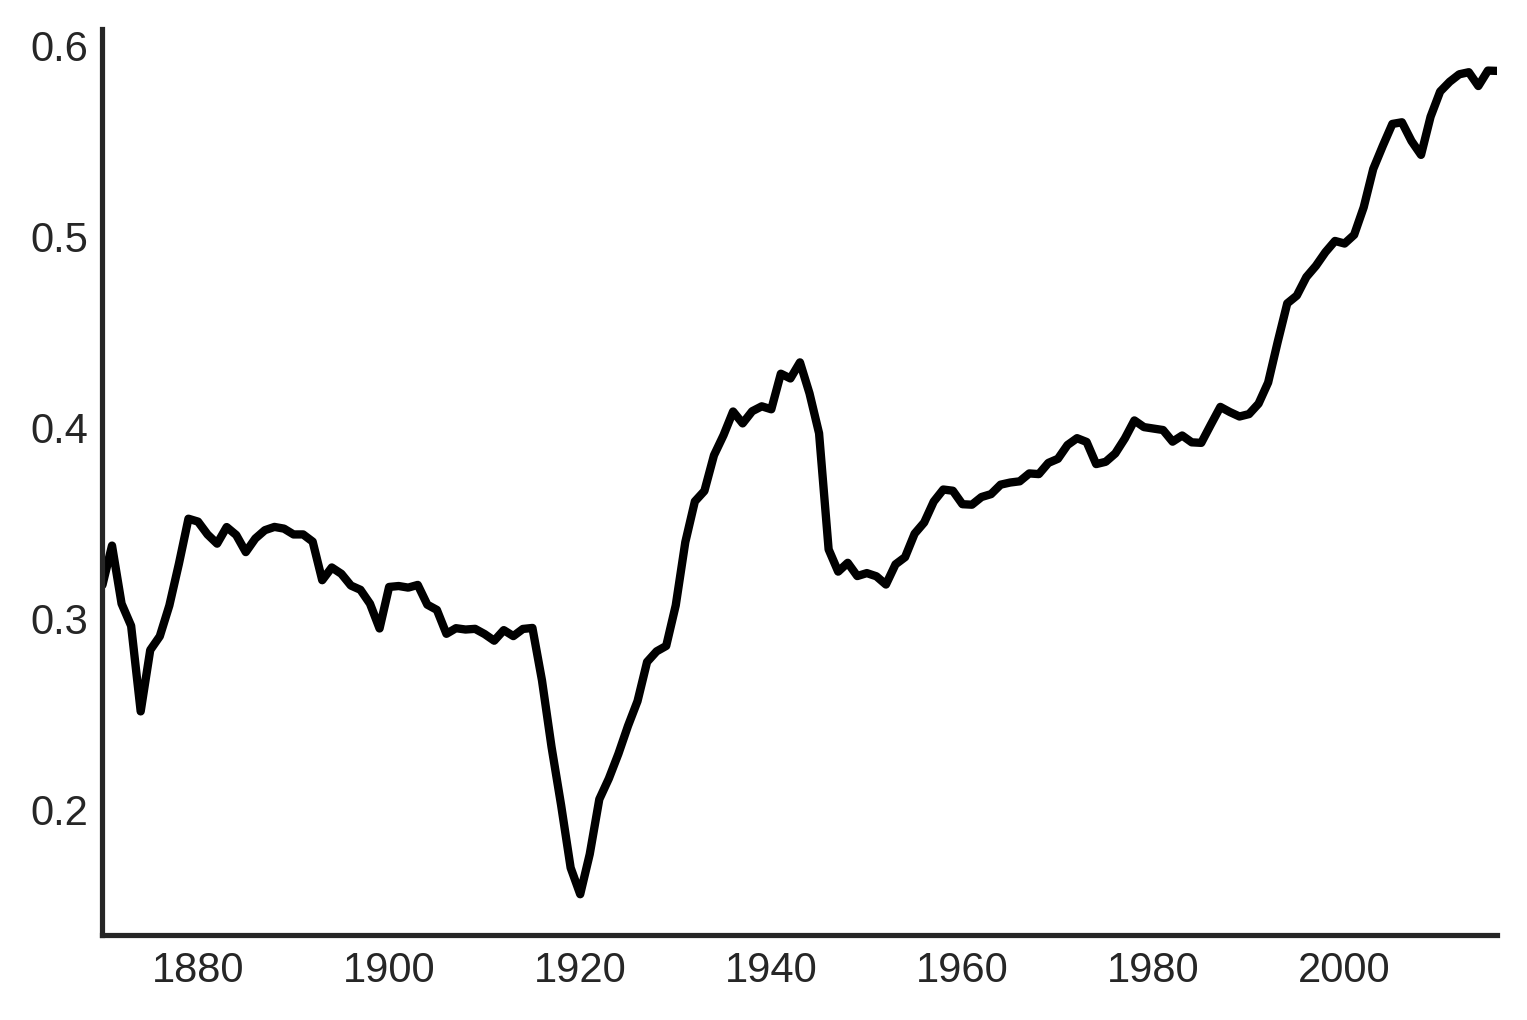
\includegraphics[width=.7\textwidth]{Jorda_Mean.png}
	\caption*{\textbf{Fonte:} \textcite[p.~10]{jorda_great_2014}}
\end{figure}


Recentemente, parte da literatura econométrica também tem lançado luz sobre a importância do investimento residencial para o ciclo econômico\footnote{Além da importância do investimento residencial para a dinâmica econômica, cabe pontuar a relevância da taxa de aquisição de imóveis na determinação do endividamento das famílias e, portanto, destacar a importância de se estudar o tema \cite{schwartz_politics_2009}.
}. \textcite{alvarez_does_2010}, por exemplo, concluem que tal tipo de investimento antecede o ciclo econômico para o caso espanhol e resultados semelhantes podem ser encontrados para França, Espanha  e Itália enquanto o caso alemão apresenta uma dinâmica distinta \cites{ferrara_cyclical_2010}{ferrara_common_2010}. 
Outros estudos empíricos, por sua vez, têm enfatizado o efeito riqueza --- via valorização dos imóveis --- sobre o consumo e indicam tais canais de transmissão são mais incidentes, em ordem, sobre Estados Unidos e Grã Bretanha e mais brandos no caso francês e alemão \cites{sastre_assessment_2010}{chauvin_wealth_2010}{bassanetti_effects_2010}{arrondel_housing_2010}.

A pluralidade de resultados reportada acima sugere que a especificidade institucional de cada país desempenha um papel central nas implicações macroeconômicas do investimento residencial e, portanto, carece de uma análise mais detalhada. A título de exemplo, \textcite{wijburg_alternative_2017} destacam que o mercado imobiliário alemão\footnote{
	\textcite{wijburg_alternative_2017} também apontam que os preços dos imóveis na Alemanha estagnaram enquanto o resto do mundo presenciou um aumento. No entanto, observa-se um movimento recente de aumento nos preços no país, indicando uma maior relevância do tema em um futuro próximo.} é um contra ponto ao ameriacano\footnote{
	A metodologia utilizada por \textcite{wijburg_alternative_2017} é a das ondas de financeirização em que a última onda iniciou no fim da CFG. Dito isso, os autores negam a ideia de que o mercado imobiliário alemão não é financeirizado uma vez que a financeirização imobiliária pode assumir várias formas.}:

\begin{quote}
	\textit{On the one hand, the German housing market was one of the few markets in Western Europe that was not severely affected by the global housing boom of the early 2000s. On the other hand, recent developments suggest that the role of finance in the German housing system is \textbf{changing}, but not in the same way as in other countries} \cite[p.~969, grifos adicionados]{wijburg_alternative_2017}
\end{quote} 


Sendo assim, cabe destacar a importância das instituições\footnote{
	Ao longo desta pesquisa, adota-se a definição de instituições como em 	\textcite[p.~85]{dequech_economic_2013}: ``\textit{Institutions are broadly understood here as socially shared systems of rules of behavior or of thought that have some recurrence}'' e, mais especificamente, serão avaliadas as instituições formais.} 
para a compreensão das inter-relações entre o mercado imobiliário e o de crédito.  
%No que diz respeito ao arranjo institucional do mercado imobiliário, seja ele micro ou macro econômico, influencia principalmente nas formas que os credores (bancos e investidores institucionais) administram o risco e os custos dos empréstimos hipotecários. 
Seguindo este tipo de análise, \textcite{van_gunten_varieties_2018} argumentam que as mudanças institucionais foram responsáveis pela maior intensificação financeira --- maior endividamento das famílias e não um aumento no número de famílias endividadas --- em Portugal e Espanha se comparado com França e Alemanha\footnote{\textcite[p.~92]{van_gunten_varieties_2018} também pontuam a especificidade do caso alemão em que houve um ``desintensificação financeira''.}. Dentre os principais determinantes institucionais a serem analisados, destaca-se: (i) possibilidade de transferência de riscos (\textit{e.g.} securitização\footnote{Para uma descrição do aumento da securitização nos Estados Unidos, ver \textcite{green_american_2005} e \textcite{cagnin_o_2009}.}) que têm aumentado entre os países europeus \cite{european_central_bank_housing_2010}; (ii) disponibilidade de crédito de longo-prazo para as famílias \cite{schwartz_politics_2009}; (iii) duração das hipotecas e existência de um mercado secundário \cite{green_american_2005}; (iv) determinação  e tipo da taxa de juros das hipotecas (fixa ou flexível); (v) arranjo regulatório sobre reembolso antecipado (contrato ou legislação) e formas de refinanciamento e; (vi) acesso a linhas de crédito, ou seja, permissividade da retirada do capital próprio (\textit{equity withdrawal contracts}). Dentre os itens elencados anteriormente (organizados na tabela \ref{Institucional} para alguns países), destaca-se o acesso a linhas de crédito através das hipotecas cuja relevância é maior para o caso norte-americano --- pelos efeitos significativos já mencionados sobre o ciclo econômico --- e por serem mais incomuns nos países europeus \cite[p.~95]{van_gunten_varieties_2018}.

\begin{table}[htb]
	\centering
	\caption{Características institucionais de alguns países europeus}
	\label{Institucional}
	\resizebox{\textwidth}{!}{%
		\begin{tabular}{l|c|c|c|c|c|c}
			\hline \hline\\
			\textbf{Fatores institucionias}                                                              & \multicolumn{1}{c}{\textbf{França}} & \multicolumn{1}{c}{\textbf{Alemanha}} & \multicolumn{1}{c}{\textbf{Itália}} & \multicolumn{1}{c}{\textbf{Holanda}} & \multicolumn{1}{c}{\textbf{Portugal}} & \multicolumn{1}{c}{\textbf{Espanha}} \\\hline
			Maturidade das hipotecas                                                                       & 19                                  & 25-30                                 & 22                                  & 30                                   & 30-40                                 & 30                                   \\\hline
			Tipo de taxa de juros                                                                        & Fixa                                & Fixa                                  & Variável                            & Fixa                                 & Variável                              & Variável                             \\\hline
			\begin{tabular}[c]{@{}l@{}}Reembolso antecipado:\\ Contrato (C)/ Legislação (L)\end{tabular} & C/L                                 & C/L                                   & L                                   & C                                    & L                                     & C/L                                  \\\hline
			\begin{tabular}[c]{@{}l@{}}Retirada de capital próprio \\ (Permissão)\end{tabular}           & Não                                 & Não                                   & Não                                 & Sim                                  & -                                     & Limitado                             \\\hline
			\begin{tabular}[c]{@{}l@{}}Financiamento pelo \\ mercado de capitais\end{tabular}            & 12\%                                & 14\%                                  & 20\%                                & 25\%                                 & 27\%                                  & 45\%                                 \\\hline
			\begin{tabular}[c]{@{}l@{}}Execução hipotecária (\textit{Foreclosure}): \\ duração (meses)\end{tabular}             & 20                                  & 9                                     & 56                                  & 5                                    & 24                                    & 8 \\ \hline\hline                                 
		\end{tabular}%
	}
\caption*{\textbf{Fonte:}  \textcite[p.~94, adaptado e traduzido]{van_gunten_varieties_2018}}
\end{table}



Pontuada a importância do investimento residencial e a relevância das instituições para compreendê-lo, cabe inspecionar a forma com que a heterodoxia tratou do tema. Parte significativa desta literatura  --- emergente no pós-crise imobiliária --- centra esforços na conexão deste tipo de gasto com processos mais gerais como a financeirização \cites{aalbers_financialization_2008}{bibow_financialization_2010} enquanto uma fração minoritária o relaciona com as variabilidades de capitalismo e as relações com o \textit{welfare state} \cite{schwartz_politics_2009}. 
No entanto, a partir da revisão bibliográfica, verificou-se que uma fração pequena da literatura heterodoxa\footnote{
	A título de menção, vale destacar também o trabalho de \textcite{zezza_u.s._2008} em que são investigados os efeitos distributivos sobre o crescimento para a economia norte-americana a partir da metodologia \textit{Stock-Flow Consistent}.}
aborda as relações entre crescimento e investimento residencial que, e isto é central para a análise, não cria capacidade produtiva ao setor privado\footnote{A título de nota, destaca-se que debate ortodoxo sobre desenvolvimento e investimento residencial centrado na década de 60-70 (ver \textcite{arku_housing_2006}) se restringiu em categorizá-lo como um gasto absorvedor de recursos produtivos e indicava  a possibilidade de um sobreinvestimento residencial \cites{solow_importance_1995}{mills_has_1987}. }. 
Uma forma de incluir esse gasto nos modelos de crescimento heterodoxos é a de \textcite{da_silveira_investimento_2019} em que os autores utilizam o supermultiplicador sraffiano (SSM em inglês) por estabelecer um papel fundamental aos gastos autônomos que não criam capacidade no crescimento econômico e na acumulação de capital\footnote{Na contribuição original de \textcite{serrano_sraffian_1995} e nas apresentações mais recentes \cite{freitas_growth_2015}, o modelo é apresentado de modo bastante parcimonioso para evidenciá-lo como um fechamento alternativo, dentro da tradição da teoria do crescimento liderada pela demanda \cite{serrano_sraffian_2017}.}. 
%Nesta família de modelos: 
%	(i) o grau de utilização converge ao normal no longo prazo; 
%	(ii) a distribuição renda tem efeitos de nível apenas e; 
%	(iii) a taxa de crescimento da economia converge a taxa de crescimento dos gastos autônomos. 


A partir do estabelecimento do SSM, algumas questões são colocadas: quais são esses gastos autônomos e quais seus determinantes? Qual o padrão de financiamento e suas consequências? \textcite{pariboni_household_2016} e \textcite{fagundes_dinamica_2017}, por exemplo, avançaram em detalhar o consumo financiado por crédito.  \textcite{brochier_supermultiplier_2018}, por sua vez, incorporam o SSM em uma estrutura contábil mais completa, o arcabouço de consistência entre fluxos e estoques (SFC, na sigla em inglês), para compreender a dinâmica do consumo a partir da riqueza. Por mais que a contribuição de \textcite{da_silveira_investimento_2019} lance luz sobre a inclusão do investimento residencial nesta família de modelos, carece de uma relação entre o mercado imobiliário e de crédito bem como uma maior ênfase no endividamento das famílias e, portanto, tal contribuição precisa ser melhor explorada e estendida.

Como será discutido adiante, a ênfase em tratar a abordagem SFC enquanto uma metodologia decorre da flexibilidade de incluir inúmeras teorias e propostas apesar da rigidez de seus procedimentos. Apenas para elencar alguns temas caros a heterodoxia, tal abordagem trata, mesmo que em sua forma mais originária\footnote{A forma originária dessa família de modelos é encontrada em \textcite{godley_macroeconomics_1983}.}, as formas de financiamento das firmas \cites{asimakopulos_kalecki_1983}{skott_finance_1988}{messori_financing_1991}; endogeneidade da moeda e importância do sistema bancário \cites{messori_financing_1991}{dow_horizontalism:_1996}{arestis_theoretical_1996}{godley_money_1999}; endividamento, distribuição de renda e, apenas para restringir os temas, financeirização \cites{palley_inside_1996}{wolfson_irving_1996}{palley_money_1997}{palley_financial_2002}{dos_santos_revisiting_2009}{palley_inside_2010}{hein_finance-dominated_2012}.

A mesma variabilidade de temas passíveis de serem abordados pela metodologia SFC se estende para a pluralidade dos ativos e do grau de complexidade financeira de cada modelo. Uma forma de visualizar tal flexibilidade é por meio da figura \ref{Heatmap} em que são mapeados os ativos mais frequentes. No entanto, este gráfico também revela que a literatura não dá a devida atenção ao investimento residencial\footnote{Deve ser pontuada a notória exceção de \textcite{zezza_u.s._2008} em que é apresentado um modelo com imóveis em um aparato Kaleckiano enfatizando as implicações distributivas mas não trata de questões envolvendo ganhos de capital ou dos determinantes do investimento residencial.}, sendo o ativo menos estudado. Portanto, fica evidenciada a lacuna que esta pesquisa procurará preencher.

\begin{figure}
	\centering
	\caption{Mapa de calor dos ativos modelados com SFC}
	\label{Heatmap}
	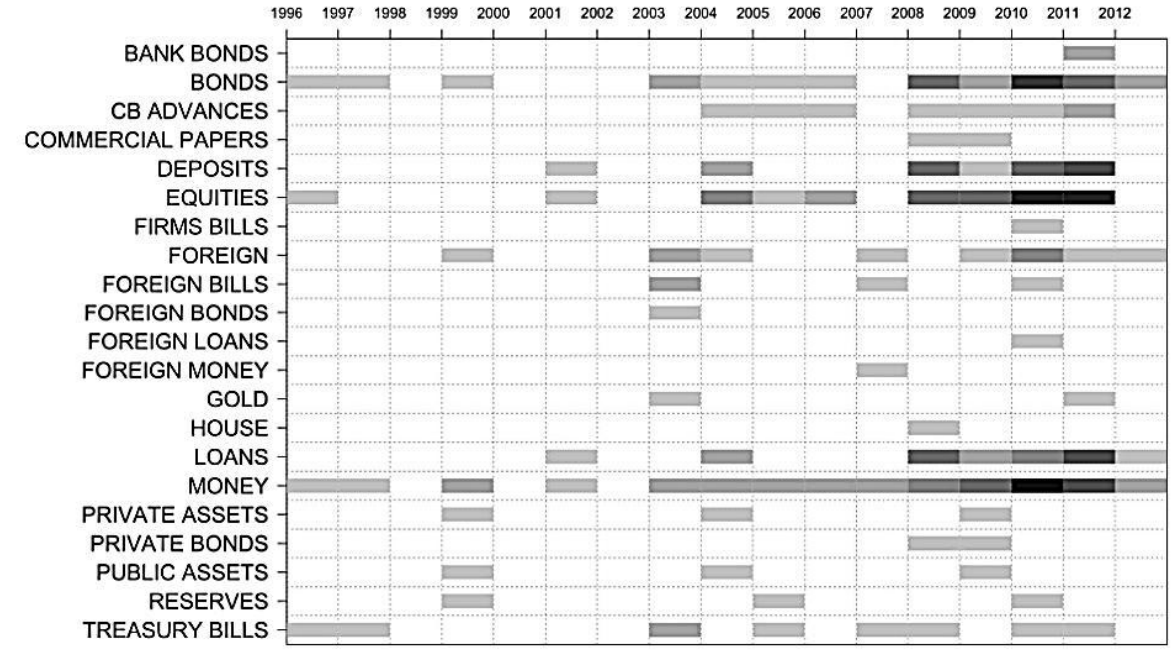
\includegraphics[width = 0.9\textwidth]{../../Escrita_Dissertacao/Da_Silveira_Dissertacao_Atual/Modelo/Caverzassi_Heatmap.png}
	\caption*{\textbf{Fonte:} \textcite[p.~4]{caverzasi_stock-flow_2013}}
\end{figure}


Uma forma de conectar o investimento residencial com o modelo do supermultiplicador sraffiano é por meio da taxa própria de juros dos imóveis (Taxa Própria) desenvolvida por \textcite{teixeira_crescimento_2015} para avaliar o caso norte americano e é definida como a taxa de juros hipotecária ($r_{mo}$) deflacionada pela inflação dos imóveis ({$\dot p_h$}) de modo que o investimento residencial, autônomo e não criador de capacidade produtiva, cresce a taxa $g_Z$ dada por:
\begin{equation}
g_Z = \phi_0 - \phi_1 \overbrace{\left(\frac{1+r_{mo}}{1+\dot p_h} - 1\right)}^{\text{Taxa Própria}}
\end{equation}
em que os $\phi_i$s são parâmetros e cujo termo em parênteses é a Taxa Própria. O primeiro parâmetro se refere aos determinantes de longo prazo (\textit{e.g.} arranjos institucionais do mercado imobiliários e de crédito) enquanto o segundo capta a demanda por imóveis decorrente das expectativas de ganhos de capital resultantes da especulação com o estoque de imóveis existente e diz respeito ao ciclo econômico.

Em outras palavras, a taxa de juros das hipotecas capta o serviço da dívida para os ``investidores'' (neste caso, famílias) enquanto a variação do preço dos imóveis permite incorporar mudança no patrimonio líquido. Portanto, aufere de modo satisfatório o custo real em imóveis de se comprar imóveis \cite[p.~53]{teixeira_crescimento_2015}. Desse modo, a partir da taxa própria de juros do imóveis é possível revelar importância do investimento residencial para além do ciclo e estendê-la para o longo prazo.  Tal proposta, portanto, lança luz sobre a influência da inflação imobiliária na construção de novos imóveis e, de acordo com o supermultiplicador sraffiano, sobre o produto como um todo. 

Como mencionado anteriormente, a referida taxa própria dos imóveis foi desenvolvida para examinar a bolha de ativos ocorria nos EUA e, portanto, não foi feita uma investigação a despeito da aplicabilidade para outros países e este é um dos objetivos desta pesquisa. Além disso, uma vez que a dívida hipotecária é o principal componente do endividamento das famílias, se faz necessária uma melhor compreensão da conexão entre o investimento residencial com as formas de financiamento e estoques financeiros de forma integrada. Nesses termos, a abordagem SFC se mostra a mais adequada para este tipo de análise. Sendo assim, um modelo de crescimento do tipo SSM com a metologia SFC (adiante, SSM-SFC) se mostra com uma alternativa para tratar do investimento residencial em que são mapeadas as relações financeiras entre os diferentes agentes institucionais.


%PERGUNTA
Compreendido este panorama, a presente investigação pretende responder a seguinte pergunta: quais os principais determinantes institucionais que explicam as especificidades do caso norte-americano frente aos demais países da OCDE a despeito das implicações macroeconômicas do investimento residencial? Como conectar o mercado imobiliário e de crédito em um modelo SSM-SFC? 
Portanto, esta pesquisa segue o caminho aberto por \textcite{brochier_supermultiplier_2018} ao adicionar um tratamento adequado das relações financeiras no SSM por meio da metodologia SFC estentendo as contribuições de: 
(i) \textcite{jorda_great_2014} ao investigar o processo de ``hipotecarização'' sob um prisma pós-keynesiano; 
(ii) \textcite{serrano_sraffian_1995} ao incluir o investimento residencial na agenda de pesquisa do supermultiplicador sraffiano; 
(iii) \textcite{teixeira_crescimento_2015} ao avaliar a aplicabilidade da taxa própria de juros para além dos Estados Unidos e;
(iv) \textcite{da_silveira_investimento_2019} ao conectar as relações entre o mercado imobiliário e de crédito diante das especificidades institucionais destacas anteriormente. 
\section{Objetivos}\label{OBJ}

\begin{description}
	\item[Objetivo geral] Investigar os arranjos institucionais do mercado imobiliário e de crédito dos países da OCDE e investigar as implicações sobre o investimento residencial e contrastá-las com o caso norte-americano
	\item[Objetivos específicos] {\color{white} Texto em branco para espaçamento}
	\begin{itemize}
		\item Examinar o processo de ``hipotecarização'' destacado por \textcite{jorda_great_2014};
		\item Comparar o caso norte-americano com os demais países da OCDE;
		\item Testar a aplicabilidade da taxa própria de juros dos imóveis desenvolvida por \textcite{teixeira_crescimento_2015} para os países da OCDE; 
		\item Detectar os principais determinantes macroeconômicos do investimento residencial por meio de um modelo de dados em painel com auxílio da base de dados desenvolvida por \textcite{jorda_great_2014};
		\item Construir um modelo SFC com supermultiplicador sraffiano cujo gasto autônomo é o investimento residencial e replicar as referidas características institucionais do mercados de crédito e imobiliário.
	\end{itemize}
\end{description}


Para atender estes objetivos, a pesquisa proposta será dividida em três frentes cada qual com seu respectivo capítulo.
A primeira delas trata da inserção e contextualização do investimento residencial em processos mais estruturais como a financeirização em contraposição a ``hipotecarização''. Para isso, serão analisadas as especificidades dos países em questão no que diz respeito ao mercado imobiliário e sua conexão com o mercado de crédito bem como a regulação de preços dos imóveis. Em outras palavras, caberá a este capítulo investigar o quão destoante é o caso norte-americano frente aos demais, com especial ênfase ao caso alemão. Compreendidas as especificidades institucionais de cada país, o capítulo seguinte irá analisar os determinantes do investimento residencial por meio de um modelo de dados em panel. Com isso, esses dois capítulos fornecem o embasamento qualitativo e quantitativo para o modelo teórico que será desenvolvido no terceiro capítulo da tese. A partir da metodologia \textit{Stock-Flow Consistent} (SFC), serão testados os diferentes arranjos institucionais destacados no capítulo primeiro bem como os determinantes do investimento residencial reportados no capítulo segundo e, assim, conectar com a literatura do supermultiplicador sraffiano. Sendo assim, cabe a seção seguinte esclarecer as etapas da metodologia SFC.

\section{Metodologia}\label{passos}

Como apresentado anteriormente, o modelo teórico é o ponto de chegada da pesquisa em que são reunidos os esforços da análise qualitativa bem como os resultados do modelo empírico. Dito isso, a presente seção ter por objetivo apresentar as etapas e procedimentos da metodologia \textit{Stock Flow Consistent} (adiante SFC\footnote{Cabe aqui destacar que tal nomenclatura decorre do trabalho de \textcite{dos_santos_keynesian_2006}.})\footnote{Para uma análise mais pormenorizada das linhagens da abordagem SFC, ver \textcite{caverzasi_stock-flow_2013}.}. Grosso modo, tal metodologia é composta de três procedimentos: (i) determinação da estrutura contábil; (ii) exposição das equações comportamentais e; (iii) solução/simulação. Dito isso, a figura \ref{Resuminho} resume as etapas mencionadas e explicitar a diferença entre a \textit{metodologia} e um \textit{modelo} SFC. 

\begin{figure}[htb]
	\caption{Resumo esquemático da Metodologia SFC}
	\label{Resuminho}
	\centering
	\begin{tikzpicture}
	[node distance = 1cm, auto,font=\footnotesize,
	% STYLES
	every node/.style={node distance=3cm},
	% The comment style is used to describe the characteristics of each force
	comment/.style={rectangle, inner sep= 5pt, text width=4cm, node distance=0.25cm, font=\scriptsize\sffamily},
	% The force style is used to draw the forces' name
	force/.style={rectangle, draw, fill=black!10, inner sep=5pt, text width=4cm, text badly centered, minimum height=1.2cm, font=\bfseries\footnotesize\sffamily}] 
	
	% Draw forces
	\node [force] (rivalry) {Equações comportamentais};
	\node [force, above of=rivalry, fill=red!70] (substitutes) {Hipóteses};
	\node [force, text width=3cm, dashed, left=1.5cm of substitutes,fill=blue!50] (state) {Metodologia SFC};
	\node [force, left=1cm of rivalry] (suppliers) {Estrutura contábil};
	\node [force, right=1cm of rivalry] (users) {Resolução};
	\node [force, right=1cm of substitutes, dashed, fill=purple!50 ] (PK) {Modelo \\SFC};
	%	\node [force, below of=rivalry] (entrants) {Threat of new entrants};
	
	%%%%%%%%%%%%%%%
	% Change data from here
	
	% RIVALRY
	\node [comment, below=0.25 of rivalry] (comment-rivalry) {Cambridge\\
		Kaleckiano\\
		\textbf{Supermultiplicador Sraffiano}};
	
	
	% SUBSTITUTES
	%\node [comment, right=0.25 of substitutes] {};
	
	% USERS
	\node [comment, below=0.25 of users] {Analítico\\
		\textbf{Simulação}};
	
	% NEW ENTRANTS
	%	\node [comment, right=0.25 of entrants] {(+) EC vs. Microsoft};
	
	% PUBLIC POLICIES
	%	\node [comment, text width=3cm, below=0.25 of state] {(1) Estrutura contábil\\
	%	(2) Equações comportamentais\\
	%	(3) \textit{Closure} do modelo};
	
	%%%%%%%%%%%%%%%%
	
	% Draw the links between forces
	\path[->,thick] 
	(substitutes) edge (rivalry)
	(suppliers) edge (rivalry)
	(rivalry) edge (users)
	(state) edge (substitutes)
	(state) edge (suppliers)
	(substitutes) edge (PK);
	
	%(entrants) edge (comment-rivalry);
	
	\end{tikzpicture} 
	\caption*{Fonte: \textcite[p.~64, adaptado]{da_silveira_politica_2017}}
	
	
\end{figure}

A ênfase em tratar a abordagem SFC enquanto uma metodologia decorre da flexibilidade de incluir inúmeras teorias e propostas apesar da rigidez de seus procedimentos. Apenas para elencar alguns temas caros a heterodoxia, tal abordagem tratar, mesmo que em sua forma mais originária\footnote{A forma originária dessa família de modelos é encontrada em \textcite{godley_macroeconomics_1983}.}, as formas de financiamento das firmas \cites{asimakopulos_kalecki_1983}{skott_finance_1988}{messori_financing_1991}; endogeneidade da moeda e importância do sistema bancário \cites{messori_financing_1991}{dow_horizontalism:_1996}{arestis_theoretical_1996}{godley_money_1999}{lavoie_note_1999}{lima_macrodynamics_2007}; endividamento, distribuição de renda e financeirização \cites{palley_inside_1996}{wolfson_irving_1996}{palley_money_1997}{palley_financial_2002}{dos_santos_revisiting_2009}{palley_inside_2010}{hein_finance-dominated_2012} e, apenas para restringir os temas; análises empíricas e proposições de política econômica \cites{godley_seven_1999}{godley_fiscal_2007}{godley_simple_2007}{arestis_income_2011}{zezza_design_2019}. 

A mesma variabilidade de temas passíveis de serem abordados pela metodologia SFC se estende para a pluralidade dos ativos e do grau de complexidade financeira de cada modelo. Uma forma de visualizar tal flexibilidade é por meio da figura \ref{Heatmap} em que são mapeados os ativos mais frequentes. No entanto, este gráfico também revela que a literatura não dá a devida atenção ao investimento residencial\footnote{Deve ser pontuada a notória exceção de \textcite{zezza_u.s._2008} e MARIA em que é apresentado um modelo com imóveis em um aparato Kaleckiano enfatizando as implicações distributivas mas não trata de questões envolvendo ganhos de capital ou dos determinantes do investimento residencial.}, sendo o ativo menos estudado. Portanto, fica evidenciada a lacuna que esta pesquisa procurará preencher.

\begin{figure}
	\centering
	\caption{Mapa de calor dos ativos modelados com SFC}
	\label{Heatmap}
	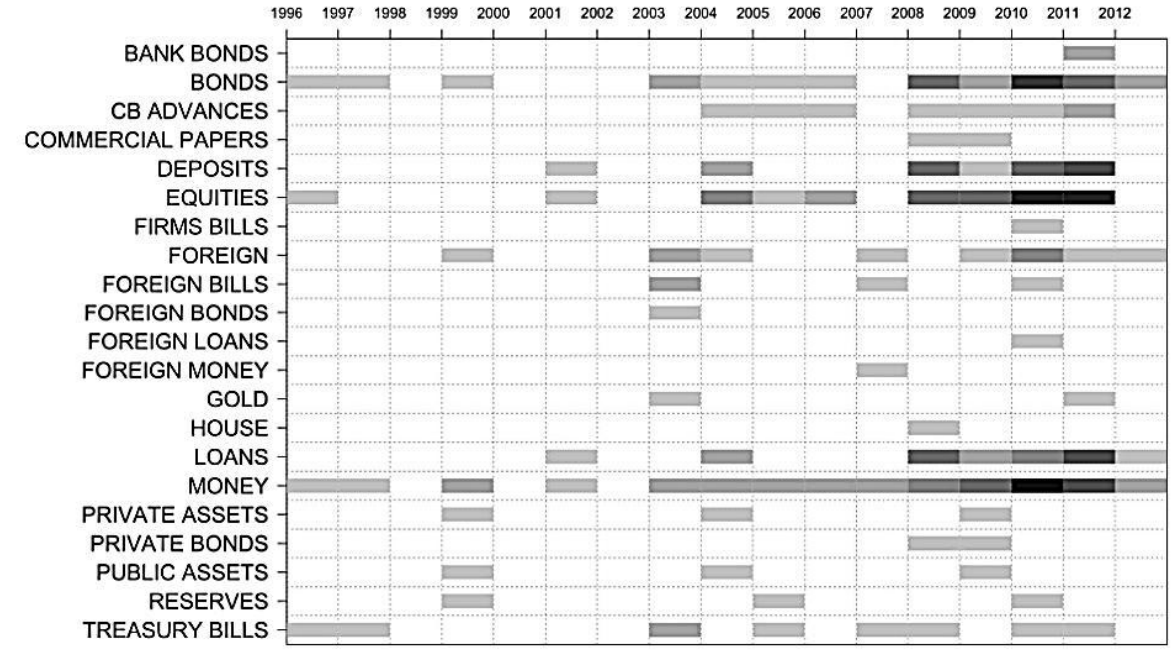
\includegraphics[width = 0.9\textwidth]{../../Escrita_Dissertacao/Da_Silveira_Dissertacao_Atual/Modelo/Caverzassi_Heatmap.png}
	\caption*{\textbf{Fonte:} \textcite[p.~4]{caverzasi_stock-flow_2013}}
\end{figure}

As etapas contábeis da abordagem SFC constituem em\footnote{Esta seção não pretende expor a metodologia pormenorizadamente, mas sim expor seus procedimentos de modo a esclarecer as etapas que foram adotadas. Para uma apresentação mais gradual, ver \textcite[Capítulo 4]{da_silveira_politica_2017}.}: (i) seleção dos setores institucionais e dos ativos a serem incorporados; (ii) mapeamento das relações dos fluxos entre os mencionados setores por meio da construção da matriz de fluxos; (iii) construção da matriz dos estoques de riqueza (real e financeira) em que são contabilizadas os ativos e passivos  bem como a posição líquida de cada setor; (iv) identificação das formas que os fluxos são financiados e sua respectiva acumulação/alocação dos estoques. Portanto, ao partir de um aparato analítico baseado em identidades macroeconômicas, surgem restrições que precisam ser seguidas.
%Vale destacar que as identidades contábeis são o ponto de partida, mas não são suficientes para garantir a consistência do modelo\footnote{Exemplo disso pode ser visto na exposição de  \textcite[p.~27--8]{godley_monetary_2007}  a despeito da contabilização das ações que não são, legalmente, um passivo das firmas e, portanto, o pagamento de dividendos não é uma obrigação contratual. Apesar disso, considera-se que as ações emitidas pelas firmas são similares aos \textit{corporate bonds}, garantindo a consistência do modelo. O que pretende ser destacado é que por mais que tal simplificação seja razoável, não deixa de ser uma hipótese.}. Para isso, é necessário que a soma da posição financeira líquida de cada setor institucional seja zero de modo que não existam ``buracos negros''. 
Tal procedimento garante que para que um setor acumule riqueza financeira, outro precisa necessariamente liquidá-la de modo que não existam ``buracos negros''.

Por mais que esta etapa é centrada nas contas nacionais, isso não implica que não possua um componente teórico associado. \textcite[p.~15--16]{macedo_e_silva_peering_2011}  pontuam que estão presentes elementos pós-keynesianos: 
(i) os agentes econômicos são categorizados de acordo com o estoque de riqueza; 
(ii) os agentes celebram contratos que impactam sua riqueza e geram fluxos monetários e implicam em mudanças na composição patrimonial desses agentes; 
(iii) ganhos e perdas de capital afetam o valor dos estoques e a dinâmica do sistema; 
(iv) a composição patrimonial dos setores institucionais evolui de forma assimétrica de acordo com o grau de alavancagem, preferência pela liquidez/risco e 
(v) o acúmulo de ativos e passivos pelos agentes interfere na correlação de forças da economia. 

Desse modo, por mais que a estrutura contábil parta das identidades, isso não a isenta de teoria. No entanto, por se tratar de identidades, nada de causal pode ser extraído delas. As relações de causalidade do modelo (agora modelo e não metodologia) decorrem das equações comportamentais que, respeitando a consistência, podem ser de qualquer linhagem teórica. Feitas essas ressalvas, dada a estrutura contábil e explicitadas as hipóteses (via equações comportamentais), resta seguir para a resolução do modelo. Como pontuam \textcite{caverzasi_stock-flow_2013}, existem duas vias: (i) simulação e (ii) descrição. A primeira delas permite expor de forma mais clara as relações entre as variáveis de modelos mais complexos em que a solução analítica não é facilmente encontrada. No entanto, tal caminho fez com que o grau de complexidade dos modelos simulados fosse exponencializada de modo que a intuição econômica torna-se facilmente turva. Diante destas complicações, a presente investigação priorizará a parcimônia de modo que serão incluídos apenas os elementos estritamente necessários para a narrativa. A justificativa desta postura decorre da maior clareza obtida sem necessariamente incorrer em um menor realismo. 

RESULTADOS ESPERADOS
%\section{Resultados esperados}\label{Result}
Realizada esta pesquisa, esperam-se os seguintes resultados:
\begin{itemize}
	\item As mudanças redistributivas observadas são relevantes para explicar a dinâmica da economia brasileira no período em questão;
	\item O crédito ao consumidor teve efeitos significativos tanto sobre o consumo de bens duráveis quanto no aumento do endividamento das famílias;
	\item O maior acesso ao crédito decorre tanto da maior participação dos salários na renda viabilizada pelas valorizações reais do salário mínimo (aumento do colateral) quanto medidas deliberadas de política econômica;
	\item Encontrar uma taxa de juros relevante ao longo prazo tal como argumentado por \textcite{pivetti_essay_1992};
	\item Espera-se destacar o conflito distributivo por meio de mudanças na taxa de juros mencionada acima para o caso brasileiro;
	\item Os componentes que explicam a dinâmica econômica do Brasil podem ser captados pelo modelo do supermultiplicador sraffiano.
\end{itemize} % Resultados esperados temporariamente desativados
\section{Plano de trabalho e cronograma de atividades}\label{cronograma}

A tabela \ref{crono} apresenta um esboço das atividades a serem desempenhadas ao longo desta pesquisa. Tendo em vista que a eventual aprovação ocorrerá quando o programa de mestrado do candidato estiver em andamento, foram destacadas em cinza as atividades que já foram desempenhadas pelo requerente. Além disso, foram destacadas em amarelo as atividades que serão executadas ao longo do período de avaliação de projetos (73 dias em média\footnote{Informação baseada no ano de 2017 e obtida no link \url{http://www.fapesp.br/estatisticas/analise/} acessado em 5 de julho de 2018}). 
Dessa forma, as células em azul correspondem às atividades a serem desenvolvidas ao longo do tempo de vigência da bolsa de auxílio. 
Dito isso, segue abaixo o cronograma mencionado:

\begin{table}[H]
	\centering
	\caption{Cronograma de atividades}
	\tiny
	\label{crono}
	\resizebox{0.8\textwidth}{!}{%
		\begin{tabular}{ll|l|l|l|l|l|l|l}
			\hline\hline
			\multicolumn{1}{c}{} & \multicolumn{8}{c}{Período} \\ \cline{2-9} 
			\multicolumn{1}{c}{\multirow{-2}{*}{Atividade}} & \multicolumn{1}{c|}{0-3} & \multicolumn{1}{c|}{3-6} & \multicolumn{1}{c|}{6-9 (Avaliação)} & \multicolumn{1}{c|}{9-12} & \multicolumn{1}{c|}{12-15} & \multicolumn{1}{c|}{15-18} & \multicolumn{1}{c|}{18-21} & \multicolumn{1}{c}{21-24} \\ \hline
			\textbf{1. Fundamentação teórica} &  \multicolumn{8}{c}{}\\ \hline
			1.1. Disciplinas &  \cellcolor[HTML]{9B9B9B} & \cellcolor[HTML]{9B9B9B} & \cellcolor[HTML]{f4df09}  & \cellcolor[HTML]{5076B0}  &\cellcolor[HTML]{5076B0}  & \cellcolor[HTML]{5076B0} &  &  \\ \hline
			1.2. Revisão bibliográfica & \cellcolor[HTML]{9B9B9B} &\cellcolor[HTML]{9B9B9B}  &\cellcolor[HTML]{f4df09}  & \cellcolor[HTML]{5076B0} & \cellcolor[HTML]{5076B0} &  &  &  \\ \hline
			\textbf{2. Análise computacional} &  \multicolumn{8}{c}{}  \\ \hline
			2.1. Pesquisa em linguagem de programação   & \cellcolor[HTML]{9B9B9B} & \cellcolor[HTML]{9B9B9B} & \cellcolor[HTML]{f4df09} & \cellcolor[HTML]{5076B0} & \cellcolor[HTML]{5076B0} &  &  &  \\ \hline
			2.2. Construção do modelo teórico &  &  &  & \cellcolor[HTML]{5076B0} & \cellcolor[HTML]{5076B0} & \cellcolor[HTML]{5076B0} &  &  \\ \hline			
			\textbf{3. Análise empírica} &  \multicolumn{8}{c}{}  \\ \hline
			3.1. Coleta de dados & \cellcolor[HTML]{9B9B9B} & \cellcolor[HTML]{9B9B9B} & \cellcolor[HTML]{f4df09} & \cellcolor[HTML]{5076B0} &  &  &  &  \\ \hline
			3.2. Simulações &  &  &  &  &  & \cellcolor[HTML]{5076B0} & \cellcolor[HTML]{5076B0} &  \\ \hline
			\textbf{4. Análise dos resultados} &  \multicolumn{8}{c}{}  \\ \hline
			4.1. Comparações com a literatura &  &  &  &  &  & \cellcolor[HTML]{5076B0} & \cellcolor[HTML]{5076B0} &  \\ \hline
			4.2. Descrição dos resultados obtidos &  &  &  &  &  & \cellcolor[HTML]{5076B0} & \cellcolor[HTML]{5076B0} &  \\ \hline
			\textbf{5. Exame de qualificação} &  &  &  &  &  &  & \cellcolor[HTML]{5076B0} &  \\ \hline
			\textbf{6. Redação da Dissertação de Mestrado} &  \multicolumn{8}{c}{}  \\ \hline
			6.1. Capítulo teórico &  &  &  & \cellcolor[HTML]{5076B0} & &  &  &  \\ \hline
			6.2. Capítulo descritivo &  &  &  &  & \cellcolor[HTML]{5076B0} & \cellcolor[HTML]{5076B0} &  &  \\ \hline
			6.3. Capítulo analítico &  &  &  &  & & \cellcolor[HTML]{5076B0} & \cellcolor[HTML]{5076B0} &  \\ \hline
			\textbf{7. Defesa} &  &  &  &  &  &  &  & \cellcolor[HTML]{5076B0} \\ \hline \hline
		\end{tabular}%
	\renewcommand{\arraystretch}{0.4}
	}
\end{table}




\begin{comment}
%==========================================================
%				Descartado
%==========================================================
% Please add the following required packages to your document preamble:
% \usepackage{multirow}
% \usepackage{graphicx}
%\begin{table}[htb]
%	\centering
%	\caption{Cronograma de atividades}
%	\label{crono}
%	\resizebox{\textwidth}{!}{%
%		\begin{tabular}{|l|l|l|l|l|l|l|l|l|}
%			\hline
%			\multicolumn{1}{|c|}{} & \multicolumn{8}{c|}{Período} \\ \cline{2-9} 
%			\multicolumn{1}{|c|}{\multirow{-2}{*}{Atividade}} & \multicolumn{1}{c|}{0-3} & \multicolumn{1}{c|}{3-6} & \multicolumn{1}{c|}{6-9} & \multicolumn{1}{c|}{9-12} & \multicolumn{1}{c|}{12-15} & \multicolumn{1}{c|}{15-18} & \multicolumn{1}{c|}{18-21} & \multicolumn{1}{c|}{21-24} \\ \hline
%			\textbf{1. Fundamentação teórica} &\cellcolor[HTML]{FE0000}  & \cellcolor[HTML]{FE0000} & \cellcolor[HTML]{FE0000} & \cellcolor[HTML]{FE0000} & \cellcolor[HTML]{FE0000} & \cellcolor[HTML]{FE0000} & \cellcolor[HTML]{FE0000} &  \\ \hline
%			1.1. Disciplinas &  \cellcolor[HTML]{9B9B9B} & \cellcolor[HTML]{9B9B9B} & \cellcolor[HTML]{9B9B9B}  & \cellcolor[HTML]{9B9B9B}  &\cellcolor[HTML]{9B9B9B}  & \cellcolor[HTML]{9B9B9B} &  &  \\ \hline
%			1.2. Revisão bibliográfica & \cellcolor[HTML]{9B9B9B} &\cellcolor[HTML]{9B9B9B}  &\cellcolor[HTML]{9B9B9B}  & \cellcolor[HTML]{9B9B9B} &  &  &  &  \\ \hline
%			\textbf{2. Análise computacional} & \cellcolor[HTML]{FE0000} & \cellcolor[HTML]{FE0000} & \cellcolor[HTML]{FE0000} & \cellcolor[HTML]{FE0000} & \cellcolor[HTML]{FE0000} &\cellcolor[HTML]{FE0000}  &  &  \\ \hline
%			2.1. Pesquisa em linguagem de programação   & \cellcolor[HTML]{9B9B9B} & \cellcolor[HTML]{9B9B9B} & \cellcolor[HTML]{9B9B9B} & \cellcolor[HTML]{9B9B9B} & \cellcolor[HTML]{9B9B9B} &  &  &  \\ \hline
%			2.2. Construção do modelo teórico &  &  &  & \cellcolor[HTML]{9B9B9B} & \cellcolor[HTML]{9B9B9B} & \cellcolor[HTML]{9B9B9B} &  &  \\ \hline			
%			\textbf{3. Análise empírica} &  &  &  &  & \cellcolor[HTML]{FE0000} & \cellcolor[HTML]{FE0000} & \cellcolor[HTML]{FE0000} &  \\ \hline
%			3.1. Coleta de dados &  &  &  &  & \cellcolor[HTML]{9B9B9B} & \cellcolor[HTML]{9B9B9B} &  &  \\ \hline
%			3.2. Simulações &  &  &  &  &  & \cellcolor[HTML]{9B9B9B} & \cellcolor[HTML]{9B9B9B} &  \\ \hline
%			\textbf{4. Análise dos resultados} &  &  &  &  &  &\cellcolor[HTML]{FE0000}  & \cellcolor[HTML]{FE0000} &  \\ \hline
%			4.1. Comparações com a literatura &  &  &  &  &  & \cellcolor[HTML]{9B9B9B} & \cellcolor[HTML]{9B9B9B} &  \\ \hline
%			4.2. Descrição dos resultados obtidos &  &  &  &  &  &  & \cellcolor[HTML]{9B9B9B} &  \\ \hline
%			\textbf{5. Exame de qualificação} &  &  &  &  &  &  & \cellcolor[HTML]{009901} &  \\ \hline
%			\textbf{6. Redação da Dissertação de Mestrado} &  &  &  &  & \cellcolor[HTML]{FE0000} & \cellcolor[HTML]{FE0000} & \cellcolor[HTML]{FE0000} &  \\ \hline
%			\textbf{7. Defesa} &  &  &  &  &  &  &  & \cellcolor[HTML]{009901} \\ \hline
%		\end{tabular}%
%	}
%\end{table}





%O cronograma \ref{crono} também mostra os grupos de atividades a serem desempenhadas, são elas: (i) fundamentação teórica; (ii) Análise computacional; (iii) Análise empírica e (iv) Redação da dissertação de mestrado. O tempo previsto para a dedicação deste grupo de atividades está destacado em vermelho. Os retângulos verdes, por sua vez, representam as obrigações institucionais: (i) Exame de Qualificação e (ii) Defesa da dissertação.

\end{comment}





\endgroup

%=====================================================================
% 							Bibliografia
%=====================================================================
%{\let\clearpage\relax \chapter{Bibliografia}}
%-----

\linespread{0.95} % Espaçamento de x*1.2cm para as referências
{\let\clearpage\relax\printbibliography}
%=====================================================================
% 							Fim do Documento
%=====================================================================
\end{document}